\documentclass[serif]{beamer}

\renewcommand\sfdefault{phv}
\renewcommand\familydefault{\sfdefault}
\usetheme{default}
\usepackage{color}
%\usepackage{pxfonts} % Or palatino or mathpazo
%\usepackage{eulervm}
\useoutertheme{default}
%\usepackage{texnansi}
\usepackage{color}
%\usepackage{marvosym}
\definecolor{bottomcolour}{rgb}{0.32,0.3,0.38}
\definecolor{middlecolour}{rgb}{0.08,0.08,0.16}
\setbeamerfont{title}{size=\Huge}
\setbeamercolor{structure}{fg=gray}
\setbeamertemplate{frametitle}[default]%[center]
%\setbeamercolor{normal text}{bg=black, fg=white}
%\setbeamertemplate{background canvas}[vertical shading]
%[bottom=bottomcolour, middle=middlecolour, top=black]
\setbeamertemplate{items}[circle]
\setbeamerfont{frametitle}{size=\huge}
\setbeamertemplate{navigation symbols}{} %no nav symbols


\usepackage{amsmath,  amsfonts, amsthm, graphicx, subfigure}
%\usepackage{biblatex}
 \usepackage{fancybox, ulem}
 \usepackage{mathtools}
 \usepackage{tabularx}
 \usepackage{tikz}
 \usepackage{movie15}
 %\bibliography{pumping_paper}
\newcommand{\p}{\partial}
\newcommand{\f}{\frac}
\newcommand{\B}{\textbf}
\newcommand{\I}{\textit}
\newcommand{\tab}{\hspace{10mm}}

 % \usetheme{Singapore}
% \usetheme{Warsaw}
  \setbeamertemplate{navigation symbols}{}
\title{Lecture 10}
\author{Austin Baird\\UNC Department of Mathematics\\UNC Department of Biology}
\date{\today} 

\begin{document}
\frame{\titlepage}

\begin{frame}
\frametitle{Summary}

Today we will: 
\ \\
\ \\
Try and understand series approximations and transforms (\textcolor{red}{Fourier Analysis!}) 
\end{frame}

%--------------------------------------------------------------------------------------------------------------------------------------------------------------------------------------------------------------------------%
\begin{frame}
\frametitle{Periodic Functions}

A period function satisfies the relationship: 

\begin{align*}
f(t+nP) &= f(t)\\
n &\in \mathcal{Z}
\end{align*}

Here the period is denoted $P$ and so this relations shows that for any chosen $n$ the graph will repeat itself with period $P$. Think of reconstructing a graph to have as large of a domain as you'd like by reflecting a function over and over again about the period!


\end{frame}


%%%%--------------------------------------------------------------------------------------------------------------------------------------------------------------------------------------------------------------------------%
%%



\begin{frame}
\frametitle{Examples} 

Periodic data = frequency analysis: 

\begin{figure}[h]
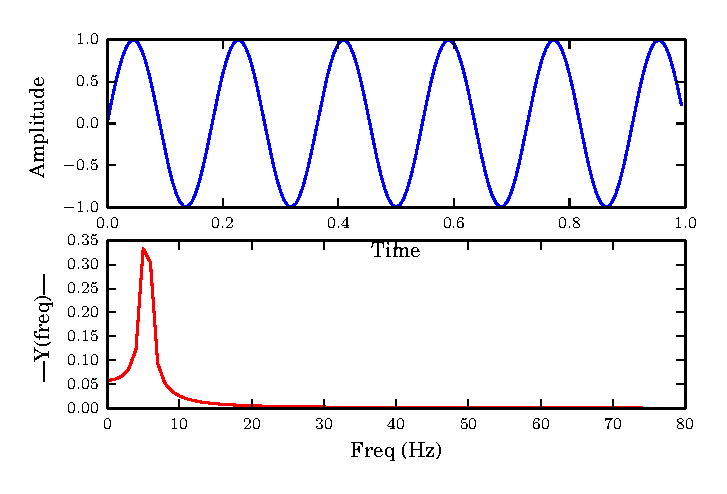
\includegraphics[width=\textwidth,height=0.7\textheight]{./freq}
\end{figure}
 

\end{frame}


%
%%%%%--------------------------------------------------------------------------------------------------------------------------------------------------------------------------------------------------------------------------%
%
\begin{frame}
\frametitle{Series Representations} 

Want to represent functions as an infinite series of terms: 

\begin{align*}
\sum_{m=0}^{\infty}a_m(x-x_0)^m 
\end{align*}

What does this look like? What is an example of this? \textcolor{red}{Taylor Series!}
\end{frame}


%%%%%--------------------------------------------------------------------------------------------------------------------------------------------------------------------------------------------------------------------------%
\begin{frame}
\frametitle{Taylor Series} 

One way to approximate functions (or not if we can deal with infinity!) is the Taylor series, defined to be: 

\begin{align*}
f(x) &= f(a) + f'(a)(x-a) + \frac{f''(a)}{2!}(x-a)^2 + \hdots\\
f(x) &= \sum_{m=0}^{\infty}\frac{f^(n)(a)}{n!}(x-a)^n
\end{align*}

This is the series representation of the function at a point $a$. 

\end{frame}

%%%%%--------------------------------------------------------------------------------------------------------------------------------------------------------------------------------------------------------------------------%
\begin{frame}
\frametitle{Homework 9}

We want to approximate functions using a discrete amount of series points! 

\begin{itemize}
\item Compute the taylor series centered at 0 for the function $\sin(x)$ (maybe by hand).
\item (to be turned in) Graph the partial sums of this series of an increasing number of terms on the same graph. 
\item (to be turned in) Qualitatively describe when these functions are no longer accurate. How far do seven terms get you? 
\item (to be turned in) Complete this experiment with $\frac{1}{1-x}$, $e^x$ are there similarities? 
\item Turn in Matlab code and a brief document of graphs and discussion (as well as the series representation of the functions). 
\end{itemize}

\end{frame}

%%%%%--------------------------------------------------------------------------------------------------------------------------------------------------------------------------------------------------------------------------%

%\begin{frame}
%\frametitle{Fourier Transform}
%
%We want to be able to transform a function from a function in terms of time or position to it's corresponding frequency domain! We will define the following transform to give us just that! 
%
%\begin{align*}
%\hat{f}(k) = \int^{\infty}_{\infty}f(x)e^{-2\pi i x k}dx
%\end{align*}
%
%With an inverse defined to be: 
%
%
%\begin{align*}
%\hat{f}(x) = \int^{\infty}_{\infty}\hat{f}(k)e^{2\pi i x k}dk
%\end{align*}
%
%Similarly we could transform a function defined with time ($t$). Also note that $k$ is the frequency of the function. 
%
%\end{frame}
%
%%%%--------------------------------------------------------------------------------------------------------------------------------------------------------------------------------------------------------------------------%
%\begin{frame}
%\frametitle{Application:}
%
%In general this this a powerful formula used to reduce PDE equations to ODEs. For example consider: 
%
%
%\begin{align*}
%\frac{\partial u(x,t)}{\partial t} = \frac{\partial u(x,t)}{\partial x}
%\end{align*}
%
%
%\end{frame}
%
%%%%--------------------------------------------------------------------------------------------------------------------------------------------------------------------------------------------------------------------------%
%\begin{frame}
%\frametitle{Discrete Transform} 
%
%Now assume that we aren't transforming a function but a sequence of data, which we know contains some oscillations: (sample the sin wave) we get: 
%
%
%\begin{align*}
%\hat{f}[k] = \sum_{n = 0}^{N-1}f[x]e^{\frac{-2\pi i k n}{N-1}}
%\end{align*}
%Here $\hat{f}[k]$ is the fourier transform of the data $f[x]$ sampled at $N$ data points. Here $k$ is the frequency. Note that $\hat{f}[k]$ is a vector of size $k$ which is the same size as the number of times we sampled the data: $f[x]$
%\end{frame}
%
%%%%%--------------------------------------------------------------------------------------------------------------------------------------------------------------------------------------------------------------------------%
%\begin{frame}
%\frametitle{More Graphs!}
%
%We can now check more parameters! 
%
%\begin{figure}
%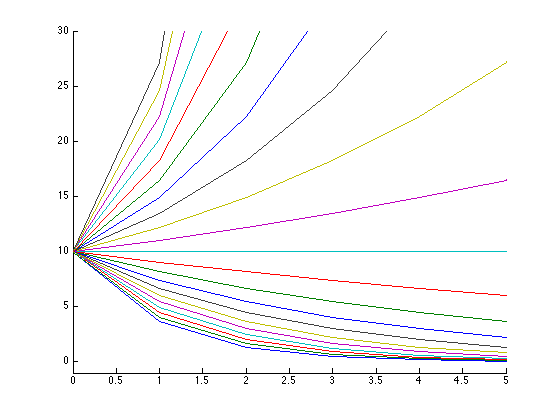
\includegraphics[width=\textwidth,height=0.7\textheight]{./exp_color}
%\end{figure}
%
%\end{frame}
%
%%%%%--------------------------------------------------------------------------------------------------------------------------------------------------------------------------------------------------------------------------%
%\begin{frame}
%\frametitle{Modeling Epidemiology} 
%
%{\tiny
%Now we want to consider tracking a disease amongst a population of individuals. Ideas modeling this (\textcolor{red}{Simple example})
%}
%\begin{itemize}
%\item People transfer from three states: Healthy $\rightarrow$ sick $\rightarrow$ healthy(immune). 
%\item \textcolor{red}{What causes the transfer between the three states?} 
%\pause 
%\item Healthy people get sick when they interact with the sick, sick people become healthy again after medicine or a period of recover time. 
%\item \textcolor{red}{What are the parameters and how do we want to denote each population?} 
%\pause 
%\item Healthy people = Susceptible ($\mathcal{S}$), sick = infected ($\mathcal{I}$), immune = removed population ($\mathcal{R}$) 
%\item Parameters: Probability of getting sick: $\alpha$, chance at each time step of recovering (if sick): $\beta$, initial populations and total population $N$.
%\item Questions: Are we adding people to the healthy population? Do immune people eventually return to susceptible? What time scale? 
%\end{itemize}
%
%
%\end{frame}
%
%%%%%--------------------------------------------------------------------------------------------------------------------------------------------------------------------------------------------------------------------------%
%\begin{frame}
%\frametitle{Writing the Equations}
%
%There are three quantities changing in time and depending on our choices previously will influence what the equations look like! \textcolor{red}{Write out your equations} 
%\pause
%\begin{align*}
%\frac{d\mathcal{S}}{dt} &= -\frac{\alpha}{N}\mathcal{S}\mathcal{I}\\
%\frac{d\mathcal{I}}{dt} &= \frac{\alpha}{N}\mathcal{S}\mathcal{I} - \beta\mathcal{S}\\
%\frac{d\mathcal{R}}{dt} &= \beta\mathcal{S}
%\end{align*}
%
%What are some parameters in this system? \textcolor{red}{Brainstorm!} How do we make this model better? \textcolor{red}{Brainstorm!}
%
%\end{frame}
%
%
%%%%%--------------------------------------------------------------------------------------------------------------------------------------------------------------------------------------------------------------------------%
%
%\begin{frame}
%\frametitle{Homework}
%{\tiny
%For the current epidemiology model: 
%}
%\begin{itemize}
%
%\item Identify important parameter values of $\alpha$ and $\beta$. What long term solutions are possible with these parameters? Does population size matter? 
%\item Compute the two parameter values from a real world scenario (choose a disease and do a bit of research on it) 
%\item Explain what is wrong with the model, are there long term solutions which can't be obtained? 
%\item \textcolor{red}{Develop a new system with the following characteristics: }
%
%\begin{itemize}
%\item Recovered population has a very slight chance of becoming susceptible again. Define the parameter value which controls this and discuss how this changes the long term behavior of the system. 
%\item Add an immunized population which susceptible can change to, should they be completely removed?. Complete the above tasks for this new population. 
%\item Add birth to the susceptible population, make the frequency be relevant to your time scales. How does this change the outcome? 
%\end{itemize} 
%\end{itemize}
%
%\end{frame}
%
%%%%%--------------------------------------------------------------------------------------------------------------------------------------------------------------------------------------------------------------------------%
%

\end{document}
